\documentclass[10pt,a4paper]{report}
\usepackage[utf8]{inputenc}
\usepackage{amsmath}
\usepackage{amsfonts}
\usepackage{amssymb}
\usepackage{graphicx}

\usepackage{hyperref}
\hypersetup{
    colorlinks,
    citecolor=black,
    filecolor=black,
    linkcolor=black,
    urlcolor=black
}

\author{Helena Brekalo}
\begin{document}


\begin{titlepage}

\newcommand{\HRule}{\rule{\linewidth}{0.5mm}} % Defines a new command for the horizontal lines, change thickness here

\center % Center everything on the page
 
\textsc{\LARGE KU Leuven}\\[1.5cm] % Name of your university/college
\textsc{\Large Ma Ingenieurswetenschappen: Computerwetenschappen}\\[0.5cm] % Major heading such as course name


\HRule \\[0.4cm]
{ \huge \bfseries Bedrijfskunde $\&$ Entrepreneurship}\\[0.4cm]
\HRule \\[1.5cm]


\textsc{\large Lesnota's}\\[0.5cm] % Minor heading such as course title


\Large \emph{Author:}\\
Helena \textsc{Brekalo}\\[3cm]

{\large 2015-2016}\\[3cm] % Date

\vfill % Fill the rest of the page with whitespace

\end{titlepage}

\tableofcontents
\clearpage

\chapter{Les 1}

\section{Slides: 1\_Bedrijfskunde\_Inleiding(1)}

\paragraph{Slide 6:} $\sim$Productlevencyclus: tijd waarin men nieuwe producten verwacht verkort $\&$ men wil steeds meer persoonlijke dingen (vari\"eteit). Zie Figuur \ref{les01_01}.

\begin{figure}[h!]
\centering
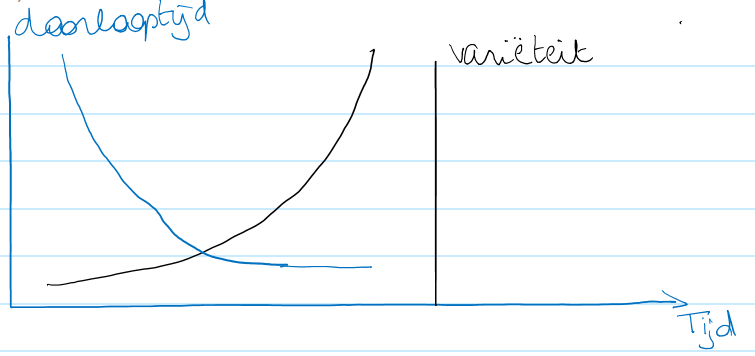
\includegraphics[width=90mm]{Les01_01.png}
\caption{Productlevencyclus} 
\label{les01_01}
\end{figure}

\paragraph{Slide 8:} Bedrijfseconomisch luik: voorspellingstechnieken: je hebt je product en je moet weten hoeveel je de komende maanden en jaren gaat produceren en welke consequenties daaraan hangen.\\
ERP: bv IER en ISP, personeelsbestanden, boekhouding,… 

\paragraph{Slide 10:} Set kleine vraagjes: vooral over begrippen (JIT, MRP,…). Let goed op verwoording en denk goed na over het antwoord! Bv: investering waarbij je 100 000 euro uitgeeft en je krijgt de volgende 5 jaar 30 000 terug, willen we nagaan of het interessant is. Als de waarde van het geld hetzelfde blijft, is het interessant. Kom niet af dat je rekenfouten gemaakt hebt op het examen!

\paragraph{Slide 13 $\&$ 14:}
\begin{itemize}
\item 5000 v.C. daar heeft men een aantal zaken teruggevonden die tonen dat men al bezig was met een soort boekhouding: bijhouden voorraden, leningen, uitgaven,… Daar werden dus al zaken opgevolgd.
\item Egyptische piramides: tonnen stenen moesten aangebracht worden, maar er waren ook enorm veel mensen aan het werken die moesten eten, slapen, verzorgd worden,…
\item 3000v.C.: volledig ontwikkeld staatssysteem.
\item Code van Hammurabi: men sprak al over minimumlonen.
\item Hannibal: logistieke organisatie om met heel die troep over te steken en eten te voorzien.
\item Feodale systemen: hi\"erarchische systemen: keizer met leenheren,… tot aan de lijfeigenen. De keizer kan niet alles voorzien dus gaat die een organisatiestructuur opbouwen die voor hem het best past. Je krijgt dan een baas die een aantal taken delegeert (bv. belastingen heffen, waarvan een deel moet worden afgestaan aan de keizer $\&$ manschappen sturen in tijden van oorlog).
\item 1300: dubbele boekhouding en kostberekeningen.
\item 1436: scheepswerf in Venetië: flowshop (alle producten volgen dezelfde weg: je hebt een aantal stations en men start met een skelet en op het einde heeft men een afgewerkte boot). Dit is zo'n bekend voorbeeld omdat er daar toen 2000 werknemers werkten en die slaagden erin om 100 boten te maken in minder dan 2 maanden. Er was dus een volledige organisatie van de lijn, de toevoer, het eten,…
\item 1700 e.v.: industri\"ele Revolutie: men bouwde stoommachines etc.: massaproductie. Men is gestart met gespecialiseerde taken, bouwmachines en massaproductie. Uitwisselbare stukken: men kan stukken gebruiken in verschillende machines: minder voorraad van die stukken nodig want je kan ze op meerdere plaatsen gebruiken. Bv kopiemachines: worden al voor 3e of 4e keer gebruikt. Zo'n 80\% van een oude machine is nog bruikbaar en wordt dus hergebruikt.
\item 1886: eerste keer ingenieur als economist $\rightarrow$ industrial engineering.
\item Henri Fayol: je moet denken aan productie, veiligheid, sturen plannen, accountancy,… $\rightarrow$ extra zaken die aan bod komen.
	\end{itemize}
	
\paragraph{Slide 15:} Ondernemen: er zijn mensen, materialen,…\\
Schumpeter: gebruikte de term ``ondernemer'' voor het eerst in de vorm van innovator. \\
Bedrijven worden alsmaar complexer $\&$ de klant komt meer centraal te staan: hij wil meer en sneller. Er wordt ook meer gekeken naar duurzame zaken. 

\paragraph{Slide 16:} Massaproductie etc kan problemen geven (realisatie) $\rightarrow$ biedt kortetermijnwinst. Er is dus langetermijnvisie nodig. \\
Henry Ford: als een bedrijf alleen maar winst wil maken, zou het eigenlijk niet mogen bestaan. Er is ook maatschappelijke bijdrage,… nodig. Toen is men de zaken anders beginnen bekijken.\\
Club van Rome: we moeten op een andere manier tewerk gaan om ervoor te zorgen dat we nog een paar 100 jaar kunnen voortgaan.

\paragraph{Slide 17:} Men moet duurzaam werken en men moet proberen voldoen aan de noden van vandaag op zo'n manier dat we de toekomst niet compromiteren.

\paragraph{Slide 19 - 22:} Veel bedrijven willen meewerken aan duurzaamheid. Als je hun jaarverslagen neemt, zie je dat ze daar ook over duurzaamheid praten.

\paragraph{Slide 23:} Een bedrijf staat niet op zichzelf dus je moet kijken naar de positie van de onderneming. Verschillende standpunten: gebruikers (mensen die producten aankopen: hebben bepaalde verwachtingen), de maatschappij (werkgelegenheid gewenst, diensten die iets voor hen doen), verwachtingen van het individu, markten (concurrenten!).\\
Een bedrijf is een economisch maar ook een sociaal systeem: zie \textbf{Slide 24:} aandachtspunten van Lotus op het sociaal systeem.

\paragraph{Slide 25:} Een bedrijf moet een meerwaarde cre\"eren, afkomstig van inkomsten en en uitgaven. Het verschil tussen beide is de meerwaarde. Je gebruikt die meerwaarde om lonen te betalen, belastingen, vergoeding voor het kapitaal, leningen $\&$ autofinanciering (kan gebruikt worden voor investeringen,…).

\paragraph{Slide 26:} Het bedrijf staat tussen leveranciers en klanten. Alle pijltjes zijn dingen die belangrijk zijn, bv levenscyclus: waar bevindt mijn product zich in de markt, wat is zijn levenscyclus?\\ Macht: ben je een grote klant van de leverancier of de enige klant? Dan kun je een aantal zaken doordrukken. Als je maar een kleine leverancier bent, dan zal dat minder zijn.

\paragraph{Slide 30:} Je kan intrapreneurship hebben (binnen een bedrijf) of erbuiten (entrepreneurship). In beide gevallen zoekt men naar innovatie. Schumpeter dacht dat dat vooral kon gevonden worden binnen bedrijven omdat er daar meer geld beschikbaar was. Dat is niet het geval. Naarmate een bedrijf groter wordt, wordt de organisatiestructuur logger en idee\"en die van werknemers komen, komen vaak niet tot ``boven''. In kleine bedrijven komt dat dus meer boven. Mensen die goede idee\"en hebben over aangepaste producten kunnen dat in een box steken in sommige bedrijven en zo gaat men die idee\"en evalueren.

\paragraph{Slide 31:} Een idee moet goed zijn en je moet ervoor zorgen dat de klant dat wil. Normaal moet het zo zijn dat jouw product het probleem van een klant oplost. Het moet een product zijn met duidelijke specificaties en het moet een potenti\"ele markt hebben. Ook rekening houden met concurrentie (bv. wasmachinetablet: vroeger was dat alleen maar in poeder en toen kwam Finish met tabletten en die begonnen 3 maand op voorhand daar reclame voor te maken. 1 week nadat het op de markt was gekomen, kwam een copycat er ook mee op de markt om dus ook een graantje mee te pikken. Het grote voordeel was dat de reclame gemaakt werd door Finish). Je moet voldoende beginkapitaal hebben (zelf hebben, binnenbrengen door investeerders aan te spreken,…). Je moet de juiste mensen aantrekken.

\section{Slides: 2\_Bedrijfskunde\_wat is een bedrijf}

\paragraph{Slide 5:} Er kunnen verschillende standpunten ingenomen worden om te kijken naar bedrijven. 

\paragraph{Slide 6:} De 4 sectoren: 2 laatste samen (tertiaire en kwartaire). De primaire sector neemt zo'n 3\% van BNP in beslag, de secundaire 33\% en de tertiaire en kwartaire de rest. De maatschappij is volledig veranderd van agrarisch naar dienstverlening.

\paragraph{Slide 7:} Je kan het bedrijf in 2 delen splitsen: goederen en diensten. De manier van werken en plannen is hier dikwijls anders. Als je kijkt naar ziekenhuizen, zij leveren ook diensten, dat is nog een stap verder dan hier. Als je naar een bank gaat voor een lening, negoti\"eer je. Als je naar een ziekenhuis gaat voor een operatie, ben je een product want je ondergaat de operatie. 

\paragraph{Slide 11 $\&$ 12:} Aangezien je niet aansprakelijk bent, word je veel meer gecontroleerd op wat je doet. 

\paragraph{Slide 13 e.v.:} Voor welk soort bedrijven.

\chapter{Les 2}

\section{Slides: 2\_Bedrijfskunde\_wat is een bedrijf}

\paragraph{Slide 19:} Onder kleine onderneming valt ook leverancier van brandstoffen (flexibeler).

\paragraph{Slide 23:} Interne jaarrekening: voor eigen gebruik.

\paragraph{Slide 24:} Marktstructuur: als je met een nieuw product op de markt wil komen, moet je rekening houden met het type markt. Als je kijkt naar volkomen concurrentie (een 100-tal spelers op de markt en de prijs wordt bepaald door de markt), als je daar op de markt wil komen, gaat niemand daar een probleem van maken (je moet gewoon zorgen dat kostprijs $>$ productieprijs). Bij een monopolie is dat anders: 1 partij bepaalt de prijs (op zo'n manier dat hij voldoende winst kan maken). Als er dan iemand op de markt komt met een gelijkaardig product, gaat de monopolist zijn prijzen laten dalen op zo'n manier dat hij bijna zeker is dat de nieuwkomer het product niet aan die prijze kan produceren (de monopolist kan in grote volumes produceren, de binnenkomer zeer waarschijnlijk nog niet). Bij een oligopolie zijn er een beperkt aantal spelers die de markt be\"invloeden. Daar binnengeraken is ook moeilijk, maar minder moeilijk dan bij een monopolie. Monopolistische concurrentie: afzetten van andere producenten door middel van productdifferentiatie.\\
$\Rightarrow$ Kijken hoe je je bedrijf moet organiseren om op de markt te kunnen komen.

\paragraph{Slide 25 e.v.:} Hoofdstuk 7 van Technische bedrijfsvoering $\&$ organisatie.

\paragraph{Slide 27:} Normaal heb je ergens een bepaalde visie, missie, strategie. Je gaat die dingen zo organiseren om je doelen te bereiken. Als je focust op verschillende producten moet je structuur dat ook weergeven.\\
Er zijn een aantal taken in verband met productie, verkoop en marketing $\rightarrow$ verantwoordelijkheden toewijzen en kijken hoe die zaken met elkaar communiceren.

\paragraph{Slide 28:} Organisatiehandleiding: taak- $\&$ functieomschrijving: elk bedrijf moet dat dus hebben. Ook bij KULeuven (onderwijsraad). Voor elke groep/functie bestaat dat. Ieder krijgt een instructieset met taken voor zijn/haar functie. Bij audits worden al die zaken ook gecontroleerd.

\paragraph{Slide 29:} Organisatieschema: bovenaan: algemeen directeur en per karakteristiek/element van het bedrijf een aantal afdelingen die uitgebouwd zijn. De personen die in een bepaalde silo zitten, gaan niet direct met andere mensen uit andere silo's spreken, dat zal via via verlopen.

\paragraph{Slide 31:} Lijnorg = volledig hi\"erarchisch. Een persoon onder een bepaalde persoon moet alleen luisteren naar die persoon en niet naar andere hogere functies waar hij/zij niet onder staat. $\rightarrow$ Duidelijke verantwoordelijkheidsbegrenzing: je gaat niet buiten je eigen gebied.

\paragraph{Slide 32:} Co\"ordinatie: als een uitvoerder naar een ``andere" baas moet gaan, zal dat via zijn baas moeten, dan naar directeur en zo naar die andere baas: grote omweg.
Zo'n structuur zal regelmatig wijzigen, is een levend organisme.\\
Omspanningsvermogen: hoeveel mensen kan ik overzien? Als je als afdelingshoofd makkelijk 15 mensen kunt opvolgen, maar als uw afdeling tot 25 mensen omvat, moet je die mss beter opsplitsen.\\
Spanwijdte: hoeveel mensen heb ik te overzien? Als spanwijdte $>$ omspanningsvermogen: beter op te splitsen.

\paragraph{Slide 33 $\&$ 34:} Speciale functie: staffunctie: ondersteunende functie (neemt zelf geen beslissingen, alleen raad en advies en schrijft documenten zodat een van de managers/directeurs dat kan gebruiken om bepaalde dingen door te drukken/voeren). Die verzamelt informatie, op systematische manier neerschrijven zodat de manager tot een besluit kan komen. Voordeel: het is nog steeds de manager/baas die beslist, de stafmederwerker neemt zelf geen beslissingen.

\paragraph{Slide 35:} Nadelen: draagt geen verantwoordelijkheden (de directeur is nog steeds de verantwoordelijke), het kan zijn dat je een fout overwicht krijgt: dat hij teveel overwicht krijgt op de manager.\\
Stafrelaties zijn voor advies, functionele relaties: diensten die dezelfde functiedeskundigheid hebben (bv. administratie). Men probeert binnen een bedrijf allemaal dezelfde documenten te gebruiken zodat die standaard zijn en makkelijk door te geven zijn zodat alles voor iedereen duidelijk is. Vroeger kon iedereen de dingen uitschrijven zoals men wou, tegenwoordig gaat dat niet meer, er zijn standaarden en het is voor iedereen hetzelfde.

\paragraph{Slide 37:} Een afdeling/bedrijf verandert qua structuur (bv. meer werknemers) en het overzien wordt misschien moeilijker. Decentralisatie is nodig wanneer dat beter past voor het type bedrijf om bepaalde zaken beter te kunnen uitvoeren. Soms is het beter eerst te decentraliseren en dan lokaal weer te centraliseren. $\rightarrow$ Je gaat alles mixen met elkaar.

\paragraph{Slide 41:} Functionele structuur: met departementen werken.

\paragraph{Slide 48:} Voordeel: groep mensen die gekoppeld zijn aan een project zelf. Nadeel: dubbele functies.

\paragraph{Slide 50:} Men laat de functionele structuur bestaan (mensen zitten in afdelingen), maar men gaat gebruik maken van die mensen op een horizontale manier. Voor projecten pikt men er dan mensen uit. Die mensen hebben nog altijd hun normale taken met daarbovenop extra taken voor het project (\textbf{Slide 53}). Matrixstructuur: verticale en horizontale taken.

\paragraph{Slide 54:} Men probeert meer en meer samen te werken (vroeger: leverancier was evil, wou gewoon winst maken). Men maakt speciale afspraken (bv. met VMI: Vendor Managed Inventory $\rightarrow$ de leverancier en het bedrijf werken samen. De leverancier weet hoeveel stukken er in het magazijn liggen en die kent het productieplan van het bedrijf (de klant) en kan zo zelf beslissen wanneer hij het magazijn gaat aanvullen wanneer dat het beste past in zijn planning. Moet er wel altijd voor zorgen dat er genoeg stukken liggen in het magazijn. De klant betaalt alleen voor wat hij gebruikt. Op die manier kan de leverancier zich beter organiseren. Bedrijven gaan elkaar soms ook overnemen om bepaalde zaken uit te voeren.\\
Horizontaal: leveranciers gaan samenwerken (bv. luchtvaartmaatschappijen: wisselstukken worden samen bekeken).

\paragraph{Slide 57:} Als je kijkt naar bedrijven, daar zijn een aantal functies (operations, marketing en finance). Die 3 moeten altijd op mekaar afgestemd zijn, anders raak je in de problemen. Bv. Apple: op een bepaald moment maakten ze reclame over het feit dat iedereen met een Apple kon werken. Dit sprak veel mensen aan en iedereen begon dat te bestellen. De computers werden geleverd (steeds met meer vertraging). Men dacht dat er een stijging ging zijn van de verkoop, maar marketing had het opgezet zonder te informeren bij de managers en financing. Men is veel gaan verkopen, maar men kon niet leveren. Er was dus geen cash flow. Men begon met de productie, maar omdat men dat te laat wist, kwam er een tekort waarbij men tot 6 maand moest wachten voor de pc geleverd kon worden.


\begin{figure}[h!]
\centering
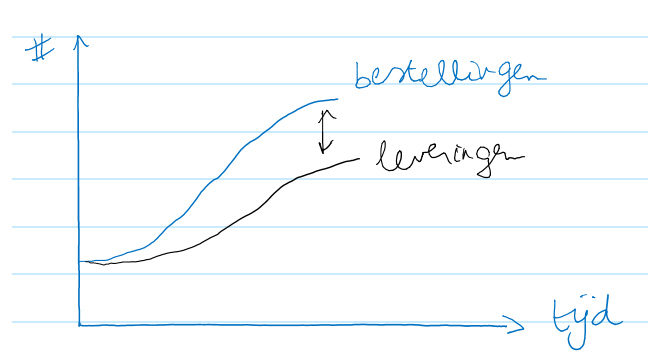
\includegraphics[width=90mm]{Les02_01.png}
\caption{Productlevencyclus} 
\label{les02_01}
\end{figure}


Dit was slechte reclame voor Apple: het was dan wel makkelijk om mee te werken, maar men moest er een half jaar op wachten.

\paragraph{Slide 58:} Bij massaproductie gaat men een lijn ontwikkelen om een bepaald product te ontwikkelen (bv. Ford Genk). Intermittent productie: het een is eenmalig, het ander is een grote batch. We hebben producten A, B, C waarbij een aantal stuks gemaakt moet worden. De productie moet zo gebeuren dat de voorraad beperkt is en de omstellingen die gemaakt moeten worden ook beperkt zijn. Je kan grote batches maken om minder omstellingen te hebben, maar dan heb je grote voorraden. Als je kleine voorraden maakt (dus kleine batches), heb je meer omstellingen en heb je te weinig tijd. De twee zijn dus tegenovergesteld aan elkaar. Je moet dit gaan optimaliseren.

\paragraph{Slide 59:} Strategische planning gaat kijken naar de impact op lange termijn (neemt niet per s\'e veel tijd in beslag!). Je moet kijken naar de tijdshorizon en zo objectieven vastleggen. Er is een hoge graad van onzekerheid omdat je over langere periodes gaat kijken, je weet niet altijd wat er juist gaat gebeuren. Het kan zijn dat men vrij goed kan voorspellen wat het verbruik gaat zijn bij klanten, maar niet per s\'e.\\
Tactische planning: wat als de verkoop cyclisch is: hoe ga je produceren? Ook cyclisch, of aan constante hoeveelheden?


\begin{figure}[h!]
\centering
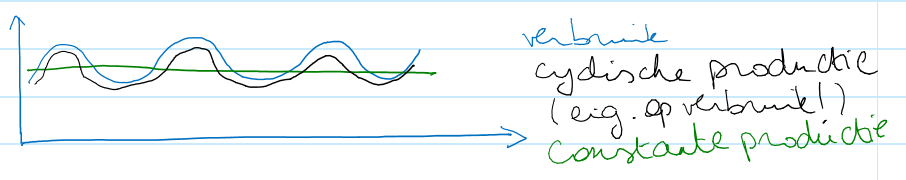
\includegraphics[width=90mm]{Les02_02.png}
\caption{Productlevencyclus} 
\label{les02_02}
\end{figure}


Normaal wordt eerst de strategische planning vastgelegd, dan tactische en dan operationele, maar het is niet puur sequentieel, het kan zijn dat men soms terugkoppelt en zaken aanpast.

\section{Slides: 3\_Bedrijfskunde\_Productlevenscyclus}

\paragraph{Slide 3:} Meestal komen producten er op basis van market pull, maar soms ook door de technologie zelf. Klanten vragen vaak zelf wel (market pull). Bij technology push gaat men proberen om noden te cre\"eren bij de klanten.

\paragraph{Slide 4:} De verschillende fasen: 
\begin{enumerate}
\item Introductie: product op de markt brengen. Hierbij is het dikwijls zo dat niemand het heeft en je moet dus zelf een prijs gaan bepalen. Als je zeker bent dat niemand het meteen gaat kopen, dan kan je de prijs relatief hoog zetten en meteen winst maken. Als het vervangbaar is door andere producten, is dat moeilijker. Als je start met een product is uw machinepark niet altijd correct afgesteld. Het product wordt dus vaak verkocht met verlies. Daarna kan je wel winst beginnen maken natuurlijk. 
\item Vroege groei: je moet nog oppassen voor copycats! 
\item Late groei: je moet je proberen differenti\"eren van andere bedrijven. Uw groei zal minder stijl zijn omdat er bv. concurrentie op de markt komt. Je zal dus minder verandering hebben, maar je moet ook kijken naar productie en financi\"en. Distributie komt hier ook bij kijken omdat je moet leveren aan de klanten.
\item Maturiteit: iedereen heeft het product en wat gekocht wordt is vervanging. Dan probeer je nog differentiatie te maken.
\item Eindstuk: iedereen is het product beu want er is een beter product op de markt, dus je kan verlies gaan lijden. Soms kan je hier geluk hebben: door je kostenstructuur te wijzigen kan je nog op een goede manier verkopen, ook als de verkoop daalt. Het kan dus zijn dat de interesse daalt, maar de marktpositie groeit nog wel.
\end{enumerate}

\paragraph{Slide 6:} Normaal, als je kijkt naar bedrijven die eerst op de markt zijn, die krijgen het grootste marktaandeel. Op de slide heb je bv. de cyclus van een bepaald product (PLC(1)), die ligt hoger dan die van PLC(2). 

\paragraph{Slide 7:} Men kan ook proberen van de levenscyclus te verlengen door er andere karakteristieken aan te geven. Bv. plakband: nieuwe versie op de markt brengen zodat het makkelijk af te scheuren is of zoiets. Zo ook met sigaretten bv. (met filter, minder teer,…).

\paragraph{Slide 8:} Niet alle curves lopen altijd hetzelfde: foothill: men brengt een product op de markt en sommige mensen moeten het dan hebben omdat het net op de markt is. Dan plots stopt het want niet iedereen is zeker of het interessant is of niet. Men wacht dan af wat de reactie is van de mensen die het al gekocht hebben. Het kan dan zijn dat het terug naar boven gaat (want positieve reacties van mensen die al gekocht hebben), of dat het niet goed is en dan daalt de curve (snel).

\paragraph{Slide 9:} Modeproducten: bv. geboorte prinses in Engeland: alle merchandise daarrond wordt enorm veel gekocht, iets later ineens niet meer. Hetzelfde verhaal met de hoolahoop.

\paragraph{Slide 10:} Grondstoffen en energiebronnen: hun gebruik is constant (olie, rubber, steenkool,…), ze zitten al lang in de maturiteitsfase.

\paragraph{Slide 11:} Als in de maturiteitsfase: flowshop maken dat specifiek gericht is op dat product. 
Je moet er rekening mee houden dat de PLC steeds korter worden, soms zijn producten al verouderd tegen dat ze op de markt komen.

\chapter{Les 3}

\section{Slides: 4\_algemene boekhouding} 

\paragraph{Slide 1} Bij een bedrijf moet je altijd een 5-jarig plan opstellen.

\paragraph{Slide 3:} We hebben een balans nodig omdat we willen weten wat er gebeurd is in het voorbije jaar. Een balans zit op strategisch niveau omdat we op lange termijn gaan kijken. Elk bedrijf moet zijn balans neerleggen bij de bank van Belgi\"e, maar vaak stelt men een tussentijdse balans op (bv. om de 3 maanden), zo kan men sneller ingrijpen indien nodig. \\
De bedoeling van algemene boekhouding is dat je ziet wat er juist gebeurd is binnen het bedrijf. Het is altijd van belang dat er een evenwicht is ($\sim$balans): we halen geld binnen (bronnen) en dat geld gebruiken we binnen ons bedrijf. De som van wat er binnenkomt moet gelijk zijn aan de som van wat we gebruiken.\\
Er zijn verschillende activiteiten die doorgaan tijdens een jaar (gewerkt, machinekosten,…) en we willen nagaan of die winstgevend zijn $\rightarrow$ resultatenrekening om te kijken of er winst gemaakt is of niet. Dan beslissen wat je met die winst gaat doen (uitkeren aan de aandeelhouders, uitgeven aan nieuwe investeringen,…).

\paragraph{Slide 4:} Figuur die het ondernemingsgebeuren weergeeft. Normaal is het zo dat als we willen produceren, we middelen moeten gebruiken om die productie te doen. Aan de ene kant interne middelen (mensen, machines) en aan de andere kant externe middelen (grondstoffen, gebruiksgoederen die zijn aangekocht). Deze middelen bepalen de kostprijs van ons product. Een deel van de middelen komt er via het verkopen van het product. Je moet weten wat de kostprijs is, welke winst je wil hebben en welke verkoopprijs je wilt. Deze laatste moet zo zijn dat je rekening houdt met uw positie in de markt.\\ Uiteindelijk komt het geld terug binnen (middelen voorgebracht door de activiteit).
Die geldstroom is enorm belangrijk: nodig om te investeren.

\paragraph{Slide 5:} We hebben een balans en resultatenrekening en we willen een samenvatting geven van wat er gebeurd is tijdens het jaar. We willen weten wat er gebeurd ismet de bezittingen en de vorderingen en het kapitaal.
Om de zaak aan te sturen zijn er de twee belangrijke principes.

\paragraph{Slide 6:} Je kan vanuit verschillende standpunten kijken naar een bedrijf (vanuit eigenaarsperspectief, banken,…).

\paragraph{Slide 7:} We hebben altijd een schuld tegenover eigenaars: zie Figuur \ref{les03_01}.

\begin{figure}[h!]
\centering
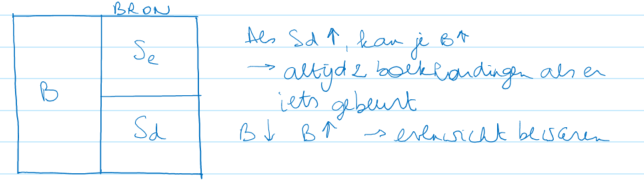
\includegraphics[width=90mm]{Les03_01.png}
\caption{Les 3 Slide 7} 
\label{les03_01}
\end{figure}

\paragraph{Slide 8:} De balans geeft altijd de zaken weer op een bepaald tijdstip (``foto"). Tussen 2 balansen (zoals hierboven getekend) heb je de resultatenrekening (geeft weer wat de activiteiten waren) en het journaal (houdt alles bij wat er gebeurt tussen 2 balansen). De balans is dus een momentopname, de resultatenrekening geeft meer de overgang aan.

\paragraph{Slide 9:} Balans: in een bepaalde volgorde (zie volgende slide). De passivazijde: staat gerangschikt volgens eisbaarheidsgraad. Het eigen vermogen is wat de personen die het bedrijf hebben opgericht hebben binnengebracht. Dat blijft in het bedrijf tot het bedrijf er eventueel mee stopt. Hoe verder naar beneden in de lijst, hoe sneller je die instantie moet terugbetalen.

\paragraph{Slide 11:} Als je kijkt naar een balans, moet dat op verschillende manieren: per kolom (anders bij dienstenbedrijven dan bij productiebedrijven). Het hangt er deels vanaf wat je gaat doen met uw winst. Je kan die bij de reserves gaan plaatsen (dan moet je die niet gaan uitbetalen), of aan dividenden (dan moet je dat uitbetalen aan de aandeelhouders). Als je de winst uitbetaalt, moet je 2000 terugbetalen op korte termijn. In principe zijn er genoeg middelen om de 2000 op korte termijn terug te betalen.
Je moet ook kijken over de tijdshorizon: naar de balans van dit jaar en van vorig jaar,… zo kan je evoluties binnen het bedrijf zien.

\paragraph{Slide 12:} Balansen van hetzelfde bedrijf, bekeken op verschillende tijdstippen. Het bedrijf werkt met seizoensgebonden vraag waarschijnlijk. Als je een piek hebt, moet je uw productieactiviteit daar niet naar aanpassen, je moet gewoon voorraad opbouwen in de magerdere periode (bv speelgoed): zie Figuur \ref{les03_02}.

\begin{figure}[h!]
\centering
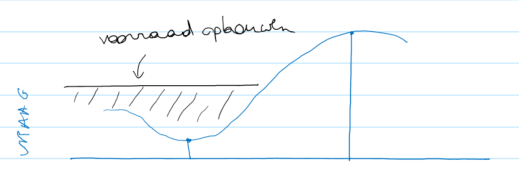
\includegraphics[width=90mm]{Les03_02.png}
\caption{Les 3 Slide 12} 
\label{les03_02}
\end{figure}

Je kan dus een totaal verschillend beeld krijgen wanneer je naar verschillende momenten in het jaar kijkt. 

\paragraph{Slide 13:} Je moet zorgen dat de balans eenduidig/juist is $\rightarrow$ wettelijke voorschriften.
\begin{itemize}
\item Informatiebron voor de bedrijfsleiding: keuzes etc.
\item Informatiebron voor diverse categorie\"en ge\"interesseerden: bv voor investeerders.
\end{itemize}
Als je een bedrijf opricht, moet je een ondernemingsplan oprichten en aantonen aan de bank dat je voldoende middelen hebt om de komende 5 jaar door te komen en dat je de interesten en aflossingen kunt afbetalen.
De overheid krijgt belastingen en als het goed gaat met het bedrijf zijn er werknemers die geen steun nodig hebben (en zij betalen ook belastingen).

\paragraph{Slide 14:} Er staan veel posten op de balans en die moeten op de juiste manier geschat worden.
\begin{itemize} 
\item Bedrijven kunnen hier laks in zijn, zeker als het gaat over financi\"ele activa (fluctueren dagelijks op de beurzen). 
\item Balanseenheid: moet eenduidig zijn en altijd hetzelfde stramien volgen. Als je lineair afschrijft (elk jaar hetzelfde bedrag), dan moet je dat elk jaar hetzelfde doen. Hetzelfde met de waardering van de voorraden. Eenmaal je gestart bent met een bepaalde regel, moet je die aanhouden $\rightarrow$ consistentie tussen verschillende balansen! Als je de regel wil aanpassen, moet je een aangepaste balans van vorig jaar geven zodat het opnieuw vergeleken kan worden.
\item Balansklaarheid: het moet duidelijk zijn wat er onder elke post staat. Als je een balans bekijkt heb je 2-3 pagina's overzicht en een 30-tal pagina's met verduidelijkingen van wat er juist bedoeld wordt.
\end{itemize}

\paragraph{Slide 15:} De sociale context is meer en meer aan het groeien.

\paragraph{Slide 17:} Zie Figuur \ref{les03_03}.

\begin{figure}[h!]
\centering
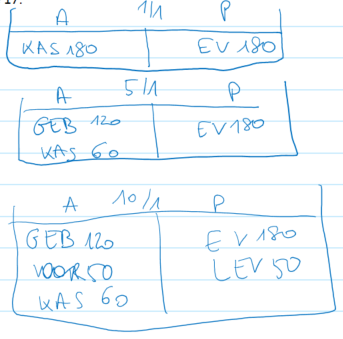
\includegraphics[width=90mm]{Les03_03.png}
\caption{Les 3 Slide 17} 
\label{les03_03}
\end{figure}

\paragraph{Slide 18:} Links altijd Debit, rechts altijd Credit (geheugensteuntje: denk aan prof zijn initialen).

\paragraph{Slide 19:} Creditzijde stijgt als we de bron laten stijgen.

\paragraph{Slide 20:} Resultatenrekening: kostenrekening en opbrengstenrekeningen: alles opgeteld. Opbrengst: credit + wat je moet aan de schuldeisers terugbetalen (je krijgt iets).

\paragraph{Slide 21:} Journaalboek waarbij alle transacties worden neergeschreven.

\paragraph{Slide 22:} Balans: alle boeken samenbrengen en alle saldi nemen en plaatsen in de balans en de resultatenrekening.

\paragraph{Slide 24 $\&$ 25:}
\begin{enumerate}
\item 2 posten: kas (dus kasboek nodig) en kapitaal.
\item Er wordt niet gespecifi\"eerd waar het geld terecht komt, dus we zetten het in de kas.
\item Er worden obligaties gekocht met geld uit de kas.
\item We hebben kosten gemaakt om producten aan te kopen, maar we hebben een voorraad en deltavoorraad liggen en 4 transacties. Alles in verband met voorraad en deltavoorraad wordt meestal apart gehouden. Wordt achteraf bekeken, rekening houdend met de waardering op dat momemt.
\end{enumerate}

Zie Figuur \ref{les03_04}, \ref{les03_05} $\&$ \ref{les03_06}.

\begin{figure}[h!]
\centering
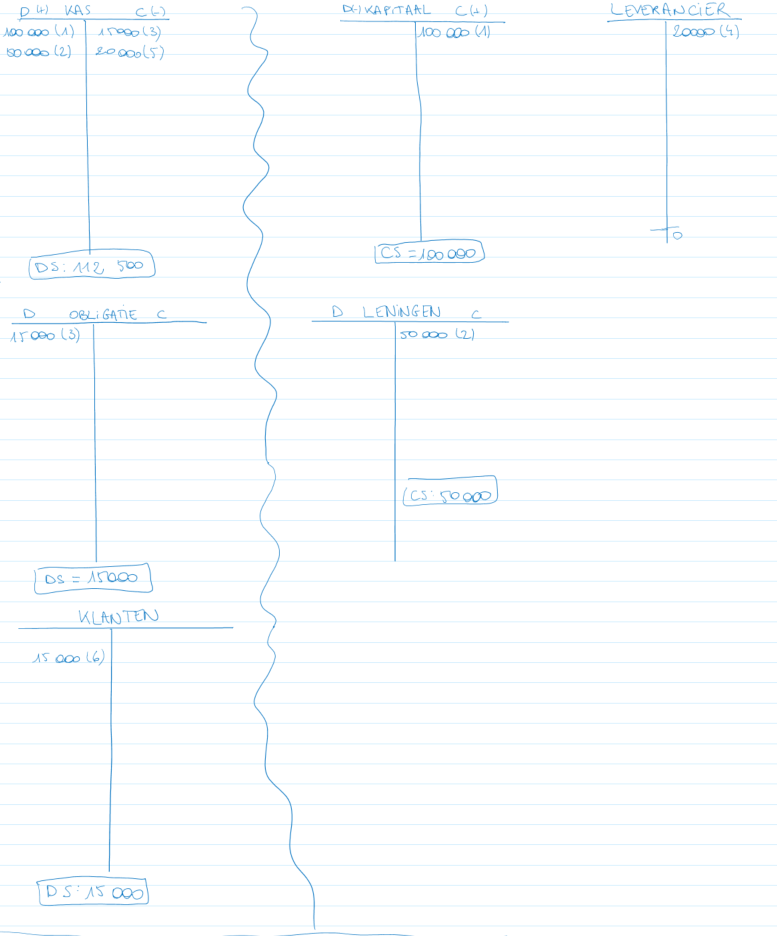
\includegraphics[width=90mm]{Les03_04.png}
\caption{Les 3 Slide 24 $\&$ 25} 
\label{les03_04}
\end{figure}

\begin{figure}[h!]
\centering
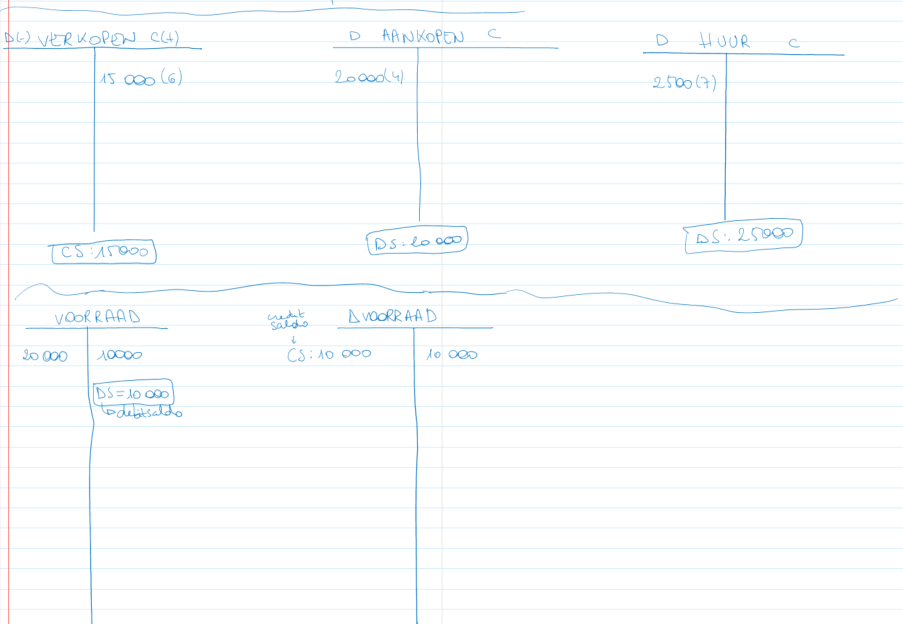
\includegraphics[width=90mm]{Les03_05.png}
\caption{Les 3 Slide 24 $\&$ 25} 
\label{les03_05}
\end{figure}

\begin{figure}[h!]
\centering
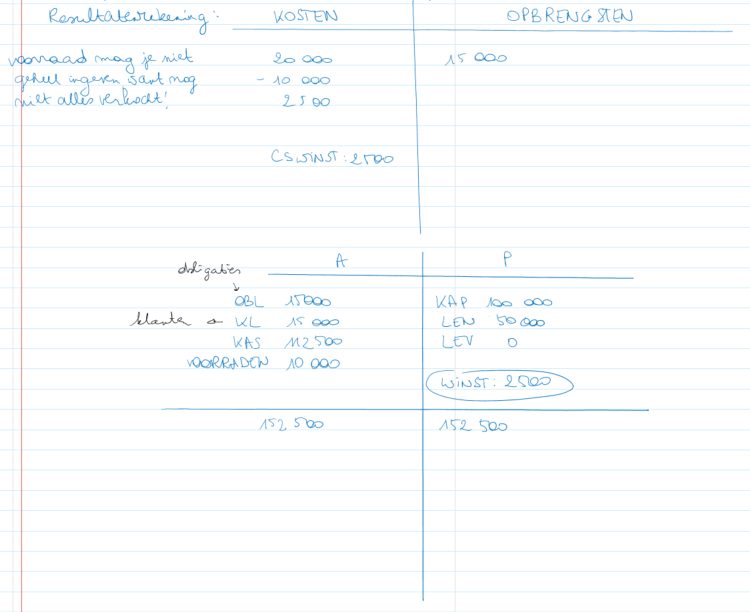
\includegraphics[width=90mm]{Les03_06.png}
\caption{Les 3 Slide 24 $\&$ 25} 
\label{les03_06}
\end{figure}

\paragraph{Slide 31:} Opgelet met voorraden: soms kan je de indruk krijgen dat je veel winst maakt terwijl dat niet zo is.

\paragraph{Slide 34:} Eerst wordt de resultatenrekening doorgerekend en dan wordt de nettowinst bekomen en die kan je opdelen in gereserveerde en verdeelde winst.

\section{Slides: 5\_Bedrijfskunde\_Financiele analyse en financiering}

\paragraph{Slide 2:} Men wil een balans tussen de eisbaarheid en de (???)graad..\\
De ratio-analyse is niet voor alle bedrijven hetzelfde, goed kijken naar de sector!\\
Financiering: we willen ervoor zorgen dat we voldoende cashflow hebben.

\paragraph{Slide 3: }
\begin{itemize}
\item Beleggers: ge\"interesseerd in beleggingen en kapitaalwinsten.
\item Schuldeisers willen hun geld terug, zijn ge\"interesseerd in rentabiliteit en de schuldenstructuur (als veel schulden: gaan niet direct willen investeren).
\end{itemize}

\chapter{Les 4}

\section{Slides: 5\_Bedrijfskunde\_Financiele analyse en financiering}
Slides: 5

Slide 4: wij gaan naar de laatste 2 kijken
Slide 5: de actiefzijde en passiefzijde wijzigen op een jaar en je wil weten hoe dat gebeurd is, welke stromen voor die veranderingen hebben gezorgd.
Slide 6: Figuur die ons vertelt hoe de kasstromen in elkaar zitten. Beneden is er de kas en daar kunnen er dingen de kas binnenkomen en verlaten
Slide 7: Als we kijken naar de balansen kunnen we ook kijken naar de mutatiebalans. We krijgen enkel de balans en geen omschrijving van wat er tijdens het jaar is gebeurd. We willen weten wat eri sgebeurd met de activa en passiva. Kijken we naar materiële vaste activa, zien we dat het bedrag met 250 gestegen is: er is een investering gebeurd (geld ergens vandaan gehaald en dat geld aangewend). Handelsvorderingen zijn ook gestegen: we verwachten nu nog meer geld terug van onze klanten (geld zit bij de klant). De voorraden zijn gedaald. Aanwending: stijging van de kosten, bron: daling.
Passiefkant: schulden op meer dan 1 jaar: die zijn gestegen: we hebben ergens meer geld binnengehaald en dat is een bron van inkomsten. De schulden < 1 jaar zijn gedaald (die zijn terugbetaald). Als een bron stijgt, stijgen de passiva.
Ook van belang is een aanwending van 250 vaste activa.
Slide 8: Let op: de totalen zijn gelijk aan die van in slide 7!
Slide 9: We gaan sterktes en zwaktes proberen afleiden obv ratio's (kerngetallen). Je kan die ratio's ook overheen de tijd bekijken en tussen verschillende ondernemingen maar wel best binnen dezelfde sector
Slide 10: We willen dat de kanten aan elkaar gelijk zijn (ook binnen de hokjes zelf, niet alleen in totaal), zo willen we bv dat we onze schulden asap kunnen terugbetalen. 
Slide 11: schulden op korte termijn terugbetaald en we hebben zo nog 80 overgehouden: er zijn reserves.
Slide 12: In slide 10 hebben we ee bedrijfskapitaal van 0 omdat we alles nodig hebben om de schulden terug te betalen. In slide 11 is het bedrijfskapitaal 80 omdat er dus nog over is.
Relatieve vorm: geeft de vergelijking aan. Als die groter is dan 1, is het bedrijfskapitaal dus positief.
Slide 13: je krijgt uw geld pas po het einde van de onderste lijn terug: je moet heel die periode dus overbruggen. Hoe langer die periode, hoe slechter voor je bedrijf. Je kan die inkorten door de productie sneller te laten worden, de voorraden kleiner te laten worden, leverancierskrediet groter te maken of het klantenkrediet kleiner te maken. Kan die periode negatief worden? Ja, bv in winkels. Bedrijven als Colruyt hebben meestal contracten van 60 tot 90 dagen (dus na 90 dagen betalen ze de leveranciers). De voorraad ligt er eestal 2 weken (dus 14 dagen). De klant betaalt meteen (dus na 14 dagen). Dit wilt zeggen dat de winkels geld hebben ontvangen voor dingen die ze zelf nog niet hebben afbetaald.



%TODO AFBEELDING





Slide 14: voorraadrotatie willen we liefst hoog, dan hebben we een kleine gemiddelde voorraad, dus deze roteert snel. We gaan de voorraad in het bedrijf inkorten (op de tekening hierboven zou het dus ook maar een aantal dagen zijn). Bv:


%TODO AFBEELDING






Klantenrotatie willen we zo klein mogelijk hebben (dan betalen ze sneller). 
Als je kijkt naar de tapijtindustrie en de voorraadperiode (VP),  het leverancierskrediet (LK) en het klantenkrediet (KK), dan liggen de tapijten er meestal 75 dagen, de leveranciers worden na 83 dagen betaald en de klanten betalen na 85 dagen. In tabelvorm:



	VP	LK	KK
Tapijt	75	83	85
Kleinhandel Voeding	29	61	10

%TODO TABEL

Slide 15: schuldenratio moet zo laag mogelijk zijn (niet teveel vertrouwen op externe financiering), solvabiliteitsratio moet zo hoog mogelijk zijn.
Toegevoegde waarde: deze wordt gebruikt om lonen te betalen, de staat te betalen,…
Slide 16: de autofinanciering is interessant: kan gebruikt worden om verdere financieringen door te voeren
Slide 17: afschrijvingen worden afgeschreven als kost maar ze zijn geen cash flow. Als je een investering doet van 1 miljoen, betaal je dat en gedurnde de volgende jaren mag je bv 100 000 afschrijven. Dit is een recuperatie van gemaakte investeringskosten, maar dat is dus geen nieuw geld dat binnenkomt.
Slide 21: grafisch voorstellen van wat daar ook staat:



%TODO AFBEELDING

























Slide 22: Balans op 31/12 die jaren x en x+1 toont.
Slide 23:






%TODO AFBEELDING





















































































Slide 25: Je moet elk jaar beslissen of je dividenden gaat uitbetalen of niet (staat dus niet vast). Obligaties moeten terugbetaald worden, aandelen niet.
Slide 26: rekening-courant: je hebt x euro staan en naarmate je daar gebruik van maakt, zoveel interest betaal je daarop



\end{document}